Certainly! Below is a TikZ LaTeX code that generates a visual representation of the described scenario. This includes both the labels for the arrow configuration at a vertex \( v \) and a sample configuration of the colored stochastic six-vertex model with \( N=2 \) and the packed boundary condition.

```latex
\documentclass{standalone}
\usepackage{tikz}

\tikzset{
    vertex/.style={circle, draw, fill=white, inner sep=5pt},
    edge/.style={->, thick},
    label/.style={below right, font=\tiny}
}

\begin{document}

% Left: Arrow configuration at a vertex v
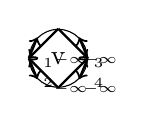
\begin{tikzpicture}[scale=1.5]
    % Vertex
    \node[vertex] (v) at (0,0) {v};
    
    % Edges and labels
    \draw[edge] (v.south) -- node[label] {$-\infty$} (v.west);
    \draw[edge] (v.south) -- node[label] {$-\infty$} (v.east);
    \draw[edge] (v.north) -- node[label] {$-\infty$} (v.west);
    \draw[edge] (v.north) -- node[label] {$-\infty$} (v.east);
    \draw[edge] (v.west) -- node[label] {$1$} (v.north west);
    \draw[edge] (v.west) -- node[label] {$2$} (v.south west);
    \draw[edge] (v.east) -- node[label] {$3$} (v.north east);
    \draw[edge] (v.east) -- node[label] {$4$} (v.south east);
\end{tikzpicture}

\hfill

% Right: Sample configuration of the colored stochastic six-vertex model with N=2 and packed boundary condition
\begin{tikzpicture}[scale=1.5]
    % Boundary conditions
    \foreach \x in {-2,-1,0,1,2} {
        \node[anchor=north, text width=2cm, align=center] at (\x,2.5) {\(\sigma(\x) = \x\)};
    }
    
    % Vertices
    \foreach \y in {0,...,3} {
        \foreach \x in